\documentclass{beamer}

\usepackage[T1]{fontenc}
\usepackage[utf8]{inputenc}

\usepackage{xspace}
\usepackage{xcolor}
\usepackage{multirow}

\usepackage{tikz}
\usetikzlibrary{arrows,snakes,backgrounds,patterns,matrix,shapes,fit,calc,shadows,plotmarks,intersections,shapes.geometric}

\usepackage{algpseudocode}
\usepackage{algorithm}

\usepackage{amsmath}
\usepackage{listings}
\definecolor{colString}{rgb}{0.6,0.1,0.1} 
\definecolor{Green}{rgb}{0.1,0.5,0.1}
\lstset{%configuration de listings 
	float=hbp,% 
	language={C},%
	morekeywords={assert, then},%
	basicstyle=\ttfamily\protect\fontsize{7pt}{7pt}\protect\selectfont, % 
	backgroundcolor=\color{white},%
	identifierstyle=\color{black}, % 
	keywordstyle=\color{blue}, % 
	stringstyle=\color{colString}, % 
	commentstyle=\color{Green}, % 
	columns=flexible, % 
	keepspaces=true,  % keeps spaces in text, useful for keeping indentation of code
	escapeinside={<@}{@>},%
	tabsize=4, % 
	frame=l, % 
	frameround=tttt, % 
	extendedchars=true, % 
	showspaces=false, % 
	showstringspaces=false, % 
	%numbers=left, % 
	numbersep=1pt,
    numberstyle=\protect\fontsize{16pt}{16pt}\protect\selectfont\ttfamily\color{black}, % 
	breaklines=true, % 
	breakautoindent=true, % 
	captionpos=b,% 
    framesep=2pt,
} 

\usepackage{pifont}% http://ctan.org/pkg/pifont
\newcommand{\cmark}{{\color{green}\ding{51}}}%
\newcommand{\xmark}{}%{\color{red}\ding{55}}}%
\newcommand{\omark}{{\color{orange}$\mathcal{O}$}}%


\usetheme{Boadilla}
\usecolortheme{dolphin}
\useoutertheme{infolines}

\beamertemplatenavigationsymbolsempty
\setbeamertemplate{footline}{
    \leavevmode%
    \hbox{%
    \begin{beamercolorbox}[wd=.25\paperwidth,ht=2.25ex,dp=1ex,center]{author in head/foot}%
        \usebeamerfont{author in head/foot}\insertshortauthor%~~\beamer@ifempty{\insertshortinstitute}{}{(\insertshortinstitute)}
    \end{beamercolorbox}%
    \begin{beamercolorbox}[wd=.5\paperwidth,ht=2.25ex,dp=1ex,center]{title in head/foot}%
        \usebeamerfont{title in head/foot}\insertshorttitle
    \end{beamercolorbox}%
    \begin{beamercolorbox}[wd=.25\paperwidth,ht=2.25ex,dp=1ex,right]{date in head/foot}%
        \usebeamerfont{date in head/foot}\insertshortdate{}\hspace*{2em}
        \insertframenumber{} / 7%\inserttotalframenumber
            \hspace*{2ex}
    \end{beamercolorbox}}%
    \vskip0pt%
}


\newcommand{\TODO}{{\color{red}\bf [TODO]}}
\newcommand{\cybersec}{cybersecurity\xspace}
\newcommand{\Cybersec}{Cybersecurity\xspace}
\newcommand{\aramis}{Aramis\xspace}
\newcommand{\DiH}{Diffie-Hellman\xspace}
\newcommand{\XOR}{Exclusive-Or\xspace}
\newcommand{\modbus}{MODBUS\xspace}
\newcommand{\opcua}{OPC-UA\xspace}
\newcommand{\ftpauth}{FTP$_{Auth}$\xspace}
\newcommand{\opcuasignenc}{OPC-UA$_{SignEnc}$\xspace}

\graphicspath{{assets/}}
\makeatletter
    \def\input@path{{assets/}}
\makeatother


\title{Formal Analysis and Smart-Fuzzing of Industrial Systems}
\author[Maxime Puys]{{\bf Maxime Puys}, Marie-Laure Potet and Jean-Louis Roch}
\institute{VERIMAG, University of Grenoble Alpes / Grenoble-INP, France\\{\texttt Firstname.Name@imag.fr}}
\date{May 10, 2016}


\begin{document}

\begin{frame}
    \maketitle

    \vspace{-3em}
    \begin{center}
        RESSI 2016
    \end{center}

    \begin{columns}
        \begin{column}{.2\textwidth}
            \resizebox{\textwidth}{!}{
                \includegraphics{logo_verimag}
            }
        \end{column}
        \begin{column}{.2\textwidth}
            \resizebox{\textwidth}{!}{
                \includegraphics{logo_uga}
            }
        \end{column}
        \begin{column}{.15\textwidth}
            \resizebox{\textwidth}{!}{
                \includegraphics{logo_inp}
            }
        \end{column}
        \begin{column}{.15\textwidth}
            \resizebox{\textwidth}{!}{
                \includegraphics{logo_pia}
            }
        \end{column}
    \end{columns}
\end{frame}

\begin{frame}
    \frametitle{Industrial Systems}

    \begin{columns}
        \begin{column}{.3\textwidth}
            \resizebox{\textwidth}{!}{
                \includegraphics{scada}
            }
        \end{column}
        \begin{column}{.3\textwidth}
            \resizebox{\textwidth}{!}{
                \includegraphics{plc}
            }
        \end{column}
        \begin{column}{.3\textwidth}
            \resizebox{\textwidth}{!}{
                \includegraphics{plant}
            }
        \end{column}
    \end{columns}
    
    \begin{block}{Hot topic}
        \begin{itemize}
            \item Increasing number of attacks showed in the medias since Stuxnet.
            \item Becoming a priority for government agencies.
            \begin{itemize}
                \item Laws to ensure the security of OIVs {\em (Loi de Programmation Militaire, Livre blanc sur la défense et la sécurité nationale, 2013)}.
                \item Publications from ANSSI {\em (Managing Cybersecurity for ICS, Protection Profils, 2012-now)}.
            \end{itemize}
        \end{itemize}
    \end{block}
\end{frame}

\begin{frame}
    \frametitle{Overview of my subject}
    
    \begin{itemize}
        \item ARAMIS Project: build a transparent device to filter industrial flows.
        \item Protocol verification: Security analysis of domain-specific protocols and configurations.
        \item Attack models: Generate attack scenarios with minimum of message to avoid IDS.
    \end{itemize}

    \begin{figure}[htb]
        \centering
        \resizebox {.7\textwidth} {!} {
            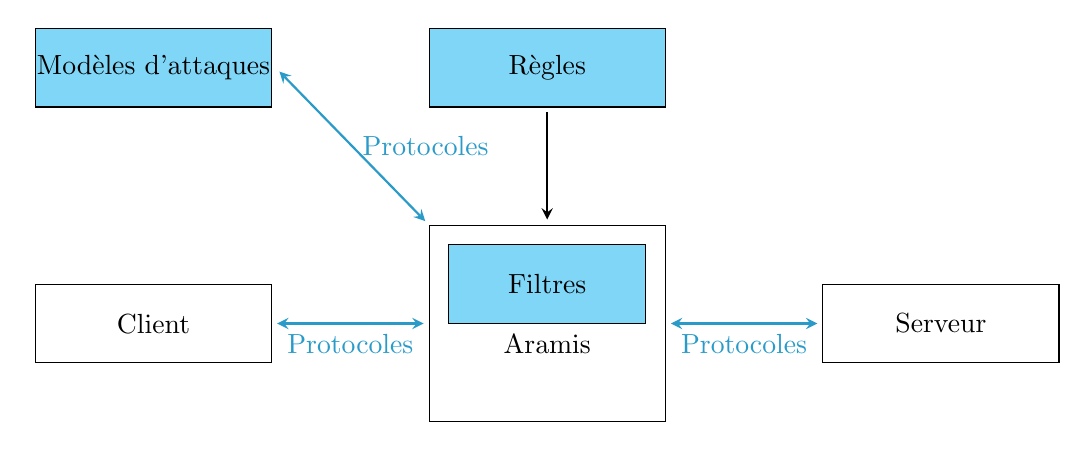
\begin{tikzpicture}[
    arrow/.style={thick,->,shorten >=2pt,shorten <=2pt,>=stealth},
    darrow/.style={thick,<->,shorten >=2pt,shorten <=2pt,>=stealth},
]

    \draw (0,.75) rectangle (3,1.75) node [pos=.5] {Client};
    
    %\fill[cyan!50!white] (5,0) rectangle (8,2.5);
    \draw (5,0) rectangle (8,2.5) node [pos=.5,below=.4] {\aramis};
    \fill[cyan!50!white] (5.25,1.25) rectangle (7.75,2.25);
    \draw (5.25,1.25) rectangle (7.75,2.25) node [pos=.5] {Filtres};
    
    \draw (10,.75) rectangle (13,1.75) node [pos=.5] {Serveur};

    \fill[cyan!50!white] (0,4) rectangle (3,5);
    \draw (0,4) rectangle (3,5) node [pos=.5] {Modèles d'attaques};

    \draw[darrow,cyan!80!black] (3.05,4.5) -- (5,2.5) node [pos=.5,right] {Protocoles};

    \fill[cyan!50!white] (5,4) rectangle (8,5);
    \draw (5,4) rectangle (8,5) node [pos=.5] {Règles};

    \draw[arrow,] (6.5,4) -- (6.5,2.5);

    \draw[darrow,cyan!80!black] (3,1.25) -- (5,1.25) node [pos=.5,below] {Protocoles};
    \draw[darrow,cyan!80!black] (8,1.25) -- (10,1.25) node [pos=.5,below] {Protocoles};

    %\draw[dashed,cyan!80!black] (-.25,-.25) rectangle (13.25,5.25);
    %\draw node [align=left,below right,cyan!80!black] at (0,5) {{\bf Attack models}};
    %\draw node [align=left,below right,cyan!80!black] at (0,4.5) {Produce attack\\scenarios given\\a system and\\attacker objectives};
\end{tikzpicture}

        }
        \caption{Axes of my thesis}
    \end{figure}
\end{frame}

\begin{frame}
    \frametitle{Overview of my subject}
    
    \begin{itemize}
        \item ARAMIS Project: build a transparent device to filter industrial flows.
        \item Protocol verification: Security analysis of domain-specific protocols and configurations.
        \item {\color{red!90!black} Attack models: Generate attack scenarios with minimum of message to avoid IDS.}
    \end{itemize}

    \begin{figure}[htb]
        \centering
        \resizebox {.7\textwidth} {!} {
            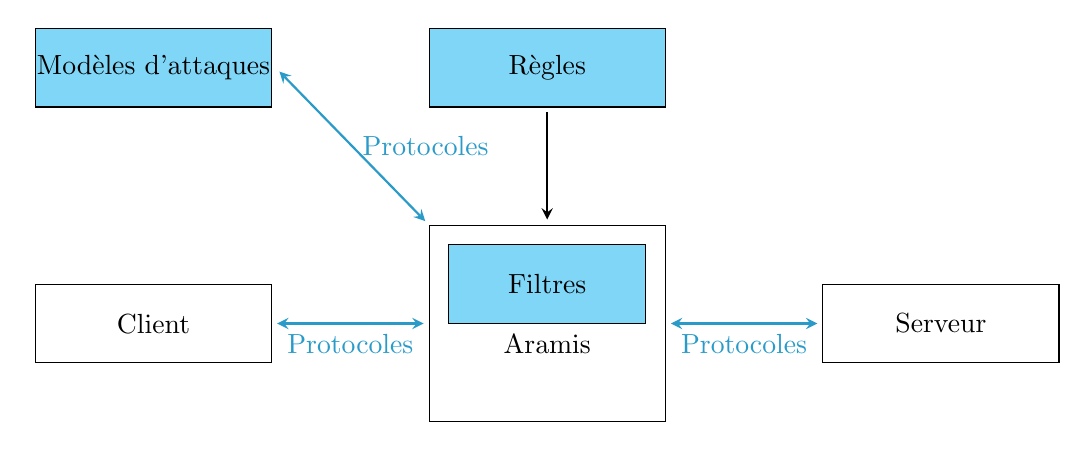
\begin{tikzpicture}[
    arrow/.style={thick,->,shorten >=2pt,shorten <=2pt,>=stealth},
    darrow/.style={thick,<->,shorten >=2pt,shorten <=2pt,>=stealth},
]

    \draw (0,.75) rectangle (3,1.75) node [pos=.5] {Client};
    
    %\fill[cyan!50!white] (5,0) rectangle (8,2.5);
    \draw (5,0) rectangle (8,2.5) node [pos=.5,below=.4] {\aramis};
    \fill[cyan!50!white] (5.25,1.25) rectangle (7.75,2.25);
    \draw (5.25,1.25) rectangle (7.75,2.25) node [pos=.5] {Filtres};
    
    \draw (10,.75) rectangle (13,1.75) node [pos=.5] {Serveur};

    \fill[cyan!50!white] (0,4) rectangle (3,5);
    \draw (0,4) rectangle (3,5) node [pos=.5] {Modèles d'attaques};

    \draw[darrow,cyan!80!black] (3.05,4.5) -- (5,2.5) node [pos=.5,right] {Protocoles};

    \fill[cyan!50!white] (5,4) rectangle (8,5);
    \draw (5,4) rectangle (8,5) node [pos=.5] {Règles};

    \draw[arrow,] (6.5,4) -- (6.5,2.5);

    \draw[darrow,cyan!80!black] (3,1.25) -- (5,1.25) node [pos=.5,below] {Protocoles};
    \draw[darrow,cyan!80!black] (8,1.25) -- (10,1.25) node [pos=.5,below] {Protocoles};

    %\draw[dashed,cyan!80!black] (-.25,-.25) rectangle (13.25,5.25);
    %\draw node [align=left,below right,cyan!80!black] at (0,5) {{\bf Attack models}};
    %\draw node [align=left,below right,cyan!80!black] at (0,4.5) {Produce attack\\scenarios given\\a system and\\attacker objectives};
\end{tikzpicture}

        }
        \caption{Axes of my thesis}
    \end{figure}
\end{frame}

\begin{frame}
    \frametitle{Attack Vectors Analysis}

    \vspace{-2em}
    \begin{columns}[c]
        \hspace{.15em}
        \begin{column}{.5\textwidth}
            \begin{figure}[htb]
                \centering
                \resizebox{\textwidth}{!}{
                    \begin{tikzpicture}[font=\Large,
    arrow/.style={thick,<->,shorten >=2pt,shorten <=2pt,>=stealth},
]
    \draw (1,1) rectangle (2,2) node [pos=.5] {$B_1$};
    \draw (3.5,1.5) circle (.5) node {$D$};

    \draw (6,0) rectangle (7,1) node [pos=.5] {$B_3$};
    \draw (6,2) rectangle (7,3) node [pos=.5] {$B_2$};
    
    \draw (0,1.5) -- (1,1.5); 
    \draw (2,1.5) -- (3,1.5); 
    \draw (4,1.5) -- (5,1.5);

    \draw (5,.5) -- (5,2.5);

    \draw (5,.5) -- (6,.5); 
    \draw (5,2.5) -- (6,2.5);

    \draw (7,.5) -- (8,.5);
    \draw (7,2.5) -- (8,2.5);
\end{tikzpicture}

                }
                \vspace{-1.8em}
                \caption{Infrastructure example}
                \label{fig:ex_archi}
            \end{figure}
        \end{column}
        \begin{column}{.6\textwidth}
            \begin{itemize}
                \item $IdTh$ = Identity theft,
                \item $AuthBP$ = Authentication by-pass,
                \item $Real(IdTh) = \{ \{ Spy \} \}$
                \item $Real(AuthBP) = \{ \{ Usurp \}, \{ Rep \} \}$
            \end{itemize}
        \end{column}
    \end{columns}
    \begin{columns}[c]
        \hspace{.5em}
        \begin{column}{.45\textwidth}
            \begin{table}[htb]
                \centering
                \begin{tabular}{|c|c|c|}
                    \hline
                    $\mathcal{R}_{Obj}$ & $IdTh$   & $AuthBP$    \\
                    \hline
                    $Client_{A}$        & \xmark    & \cmark     \\
                    \hline
                    $Router_{A}$        & \cmark    & \xmark     \\
                    \hline
                \end{tabular}
                \caption{Objectives for each attacker}
                \label{tab:ex_robj}
            \end{table}
        \end{column}
        \begin{column}{.55\textwidth}
            \begin{table}[htb]
                \centering
                \begin{tabular}{|c|c|c|c|}
                    \hline
                    $Vect$          & $Spy$     & $Usurp$   & $Rep$     \\
                    \hline
                    \ftpauth        & \cmark    & \xmark    & \cmark    \\
                    \hline
                    \opcuasignenc   & \xmark    & \xmark    & \xmark    \\
                    \hline
                \end{tabular}
                \caption{Atk. vectors for each protocol}
                \label{tab:ex_cap}
            \end{table}
        \end{column}
    \end{columns}
    \begin{columns}[c]
        \begin{column}{.55\textwidth}
            \begin{itemize}
                \item $\mathcal{S}_{Client_{A},\text{\ftpauth}} = \{ (AuthBP, Rep) \}$
                \item $\mathcal{S}_{Client_{A},\text{\opcuasignenc}} = \emptyset$
            \end{itemize}
        \end{column}
        \hspace{-1em}
        \begin{column}{.5\textwidth}
            \begin{itemize}
                \item $\mathcal{S}_{Router_{A},\text{\ftpauth}} = \{ (IdTh, Spy) \}$
                \item $\mathcal{S}_{Router_{A},\text{\opcuasignenc}} = \emptyset$
            \end{itemize}
        \end{column}
    \end{columns}
\end{frame}

\begin{frame}[fragile]
    \frametitle{Global Approach}
                    
    \begin{itemize}
        \item From modeling, automatically produce abstract attack scenarios.
        \item Convert them to real network packets with using infrastructure's context to verify and quantify their plausibility.
    \end{itemize}

    \begin{columns}[c]
        \begin{column}{.5\textwidth}
            \begin{figure}[htb]
                \resizebox{.95\columnwidth}{!}{
                    \begin{tikzpicture}[
        arrow/.style={thick,->,shorten >=2pt,shorten <=2pt,>=stealth},
    ]
    \draw (6,18) rectangle (15,21) node [pos=.5] {Infrastructure};
    \draw (18,18) rectangle (30,21) node [pos=.5,align=center] {Domain-Specific\\Security properties};

    \draw (12,12) rectangle (21,15) node [pos=.5] {Analysis};

    \draw (0,6) rectangle (9,9) node [pos=.5] {Library};
    \draw (12,0) rectangle (21,3) node [pos=.5] {Packets};
    \draw (24,6) rectangle (33,9) node [pos=.5] {Context};

    \draw (12,6) rectangle (21,9) node [align=center,pos=.5] {Instanciation\\Concretization};

    \draw[arrow] (10.5,18) -- (16.5,15); % Archi --> Analyses
    \draw[arrow] (22.5,18) -- (16.5,15); % Props --> Analyses
    \draw[arrow] (16.5,12) -- (16.5,9) node [pos=.5,right] {Set of attack scenarios}; % Analyses --> Inst
    \draw[arrow] (9,7.5) -- (12,7.5); % Biblio --> Inst
    \draw[arrow] (24,7.5) -- (21,7.5); % Context--> Inst
    \draw[arrow] (16.5,6) -- (16.5,3); % Inst --> Packets
\end{tikzpicture}

                }
                \vspace{-.25em}
                \caption{Our global approach}
            \end{figure}
        \end{column}
        \begin{column}{.5\textwidth}
            \begin{figure}[htb]
\begin{lstlisting}
Cli = cCE!0xcafe -> cCE?0xcafe -> OK
<@\vspace{-.5em}@>
E = cCE?M -> if M==0xcafe then cES!0xdead
             else cES!M -> cES?M ->
             if M==0xdead then cCE!0xcafe
             else cCE!M
<@\vspace{-.5em}@>
Srv = cES?M -> if M==0xdead then BAD -> cES!M
<@\vspace{-.5em}@>
Sys = Cli [|cCE|] E [|cES|] Srv
<@\vspace{-.5em}@>
assert Sys =\=> (BAD and OK)
\end{lstlisting}
                \vspace{-1em}
                \caption{Modeling example (CSP-like)}
            \end{figure}
            \vspace{-1.5em}
            \begin{figure}[htb]
                \resizebox{.95\columnwidth}{!}{
                    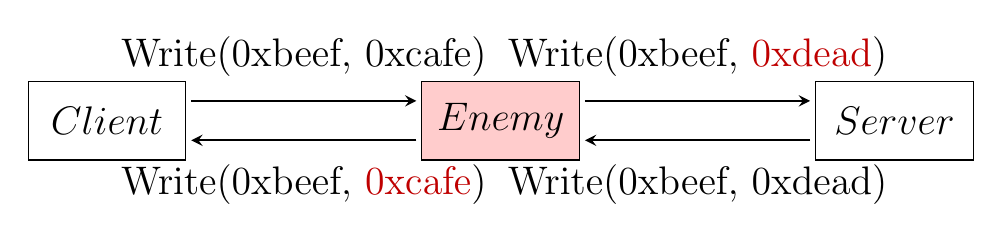
\begin{tikzpicture}[font=\Large,
    arrow/.style={thick,->,shorten >=2pt,shorten <=2pt,>=stealth},
]
    \draw (0,0) rectangle (2,1) node [pos=.5] {$Client$};
    \draw[fill=red!20!white] (5,0) rectangle (7,1) node [pos=.5] {$Enemy$};
    \draw (10,0) rectangle (12,1) node [pos=.5] {$Server$};

    % Clients - Servers links
    \draw[arrow] (2,.75) -- (5,.75)  node [anchor=south, pos=.5, align=center, above=.5em] {Write(0xbeef, 0xcafe)};
    \draw[arrow] (7,.75) -- (10,.75) node [anchor=south, pos=.5, align=center, above=.5em] {Write(0xbeef, {\color{red!75!black} 0xdead})};
    \draw[arrow] (10,.25) -- (7,.25)   node [anchor=north, pos=.5, align=center, below=.5em] {Write(0xbeef, 0xdead)};
    \draw[arrow] (5,.25) -- (2,.25)    node [anchor=north, pos=.5, align=center, below=.5em] {Write(0xbeef, {\color{red!75!black} 0xcafe})};
\end{tikzpicture}

                }
                \vspace{-.5em}
                \caption{Attack example}
            \end{figure}
        \end{column}
    \end{columns}
\end{frame}

\begin{frame}
    \frametitle{Conclusion}

    \begin{itemize}
        \item Three complementary axes:
        \begin{itemize}
            \item Attack models exploits various parameters such as security properties of protocols which shall be proved using verification tools.
            \item ARAMIS filter shall be tested against attack scenarios found by our analysis to check if they are getting fixed.
        \end{itemize}
    \end{itemize}

    \begin{itemize}
        \item Perspectives:
        \begin{itemize}
            \item Tighten bonds between attack vector analysis and global approach.
            \item Attack vector analysis could be applied to the inner-workings of the ARAMIS filter itself.
        \end{itemize}
    \end{itemize}
    
    \bigskip
    \begin{center}
        Thanks for your attention!
    \end{center}
\end{frame}

\begin{frame}
    \frametitle{Safety and Security 1/2}

    \begin{figure}[htb]
        \resizebox{\columnwidth}{!}{
            \def\rectangle{(-.5,-1.5) rectangle (4,1.75)}
\def\secondcircle{(0:5.25) ellipse (2 and 1.5)}
\def\thridcircle{(0:-1.75) ellipse (2 and 1.5)}
\def\fourthcircle{(0:1.75) ellipse (2.25 and 1)}

\begin{tikzpicture}
    \draw \rectangle node at (1.75,1.33) {Industrial systems};
    \draw \secondcircle node {\Cybersec};
    \draw \thridcircle node {Safety};
    \draw \fourthcircle node [align=center]{Industrial \\ systems \\ \cybersec};
    \begin{scope}[fill opacity=0.25]
        \fill[blue]   \rectangle;
        \fill[red]    \secondcircle;
        \fill[green]  \thridcircle;
        \fill[yellow] \fourthcircle;
    \end{scope}
\end{tikzpicture}

        }
        \caption{Relations among security concepts}
    \end{figure}
\end{frame}

\begin{frame}
    \frametitle{Safety and Security 2/2}
    
    \begin{figure}[htb]
        \resizebox{.6\columnwidth}{!}{
            %\includegraphics{liens_safety_secu}
            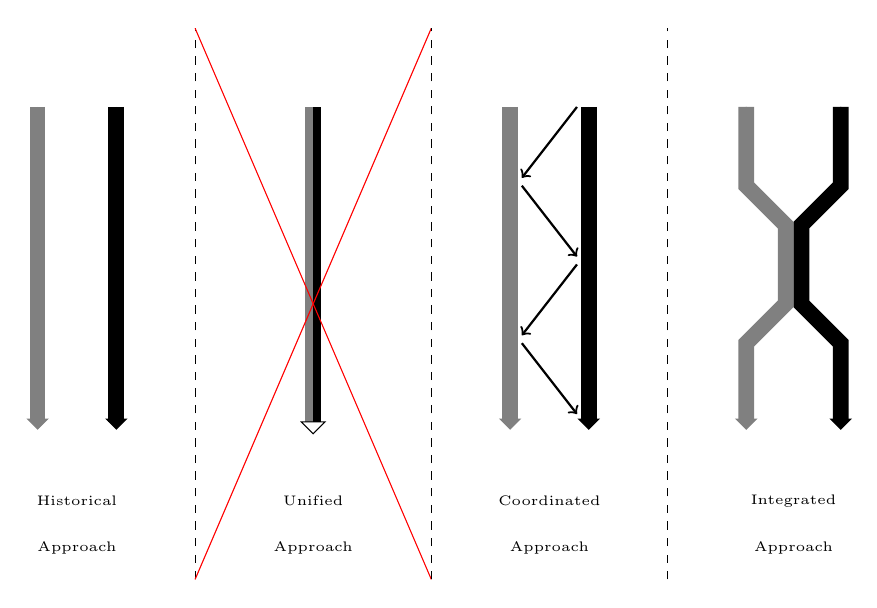
\begin{tikzpicture}[
    myarrow/.style={
        draw=black,solid,line width=2mm, postaction={-triangle 90,thin,draw,shorten >=-1mm}
}]
    %\draw[->, very thick] (0,0) -- (0,-1) -- (1,-1.5) -- (1,-2.5) -- (0,-3);
    \path[myarrow, gray] (0,5) -- (0,1);
    \path[myarrow] (1,5) -- (1,1);
    \draw node [align=center] at (.5,0) {\tiny Historical};
    \draw node [align=center] at (.5,-.6) {\tiny Approach};

    \draw[dashed] (2,-1) -- (2,6);

    \fill[gray] (3.4,1) rectangle (3.5,5);
    \fill[black] (3.5,1) rectangle (3.6,5);
    \draw (3.35,1) -- (3.65,1) -- (3.5,.85) -- cycle;
    \draw node [align=center] at (3.5,0) {\tiny Unified};
    \draw node [align=center] at (3.5,-.6) {\tiny Approach};

    \draw[red] (2,-1) -- (5,6);
    \draw[red] (5,-1) -- (2,6);

    \draw[dashed] (5,-1) -- (5,6);
    
    \path[myarrow, gray] (6,5) -- (6,1);
    \path[myarrow] (7,5) -- (7,1);
    \draw[->,thick] (6.85,5) -- (6.15,4.1);
    \draw[->,thick] (6.15,4) -- (6.85,3.1);
    \draw[->,thick] (6.85,3) -- (6.15,2.1);
    \draw[->,thick] (6.15,2) -- (6.85,1.1);
    \draw node [align=center] at (6.5,0) {\tiny Coordinated};
    \draw node [align=center] at (6.5,-.6) {\tiny Approach};

    \draw[dashed] (8,-1) -- (8,6);
    
    \path[myarrow, gray] (9,5) -- (9,4) -- (9.5,3.5) -- (9.5,2.5) -- (9,2) -- (9,1);
    \path[myarrow] (10.2,5) -- (10.2,4) -- (9.7,3.5) -- (9.7,2.5) -- (10.2,2) -- (10.2,1);
    \draw node [align=center] at (9.6,0) {\tiny Integrated};
    \draw node [align=center] at (9.6,-.6) {\tiny Approach};
\end{tikzpicture}

        }
        \caption{How to link safety and security \cite{Pie10}}
    \end{figure}
\end{frame}

\begin{frame}
    \frametitle{Purdue Model}

    \begin{figure}[htb]
        \resizebox{.8\columnwidth}{!}{
            \def\levelPhy{\small 0. Physical process}
\def\levelAut{\small 1. Automata controling the process}
\def\levelSup{\small 2. SCADA: supervision and control}
\def\levelOpp{\small 3. Production management}
\def\levelBus{\small 4. Business level, classical IT}

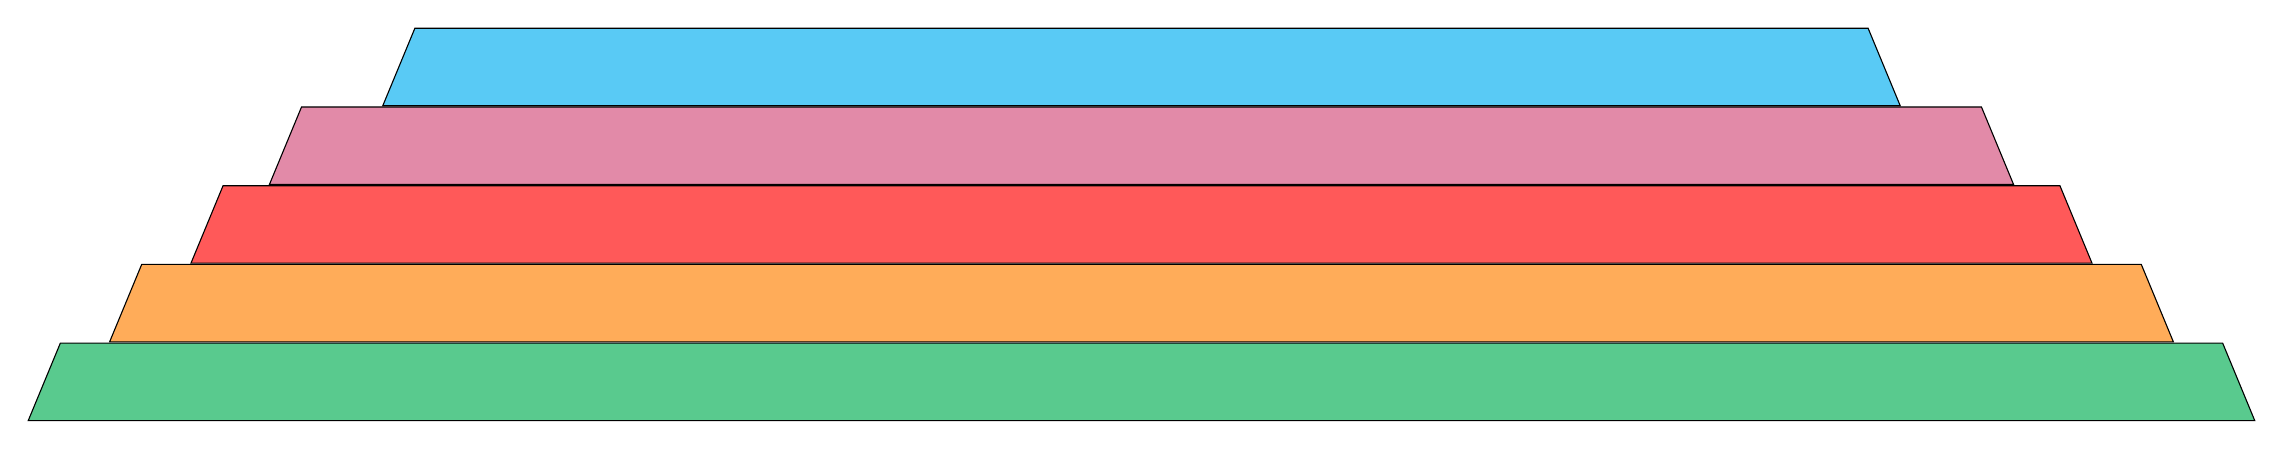
\begin{tikzpicture}[
    mytrap/.style={
    trapezium, trapezium angle=67.5, draw,inner xsep=0,outer sep=0,
    minimum height=28, text width=#1,align=center
}]

\begin{scope}[fill opacity=0.65]
        \foreach \ancho/\T/\C [count=\xi] in {186/\levelPhy/green!68!blue,172/\levelAut/orange,158/\levelSup/red,144.5/\levelOpp/purple!70,125/\levelBus/cyan}
            \node [mytrap=\ancho,fill=\C] at (0,\xi) [text opacity=1] {\T};
    \end{scope}
\end{tikzpicture}

        }

        \caption{Purdue model \cite{Wil91}}
    \end{figure}
\end{frame}

\begin{frame}
    \frametitle{Cryptographic Protocols Verification}

    \begin{exampleblock}{Needham-Schroeder}
        \vspace{-.8em}
        \begin{columns}
            \begin{column}{.45\textwidth}
            \begin{enumerate}
                \item A $\rightarrow$ B : $\{A,N_{A}\}_{KB}$
                \item B $\rightarrow$ A : $\{N_{A},N_{B}\}_{KA}$
                \item A $\rightarrow$ B : $\{N_{B}\}_{KB}$
            \end{enumerate}
            \end{column}
            ~
            \begin{column}{.45\textwidth}
                Designed and {\bf proved} in 1978.\\% by Roger Needham and Michael Schroeder.\\
                Broken in 1996 (17 years after).\\% by Gavin Lowe using \casperfdr, known as {\em Man-In-The-Middle} attack.\\
            \end{column}
        \end{columns}
    \end{exampleblock}

    \begin{exampleblock}{Man-In-The-Middle attack}
        \vspace{-.8em}
        \begin{columns}
            \begin{column}{.45\textwidth}
                \begin{enumerate}
                    \item A $\rightarrow$ I : $\{A,N_{A}\}_{KI}$
                    \item[]
                    \item[]
                          \setcounter{enumi}{1}
                    \item I $\rightarrow$ A : $\{N_{A},N_{B}\}_{KA}$
                    \item A $\rightarrow$ I : $\{N_{B}\}_{KI}$
                    \item[]
                \end{enumerate}
            \end{column}
            ~
            \begin{column}{.45\textwidth}
                \begin{enumerate}
                    \item[]
                          \setcounter{enumi}{0}
                    \item I $\rightarrow$ B : $\{A,N_{A}\}_{KB}$
                    \item B $\rightarrow$ I : $\{N_{A},N_{B}\}_{KA}$
                    \item[]
                    \item[]
                          \setcounter{enumi}{2}
                    \item I $\rightarrow$ B : $\{N_{B}\}_{KB}$
                \end{enumerate}
            \end{column}
        \end{columns}
    \end{exampleblock}
    \vfill
    \begin{itemize}
        \item Way too much possible combinations.% outpaces the humans' capabilities.
        \begin{itemize}
            \item Need of automation using tools.
        \end{itemize}
    \end{itemize}
\end{frame}

\begin{frame}[allowframebreaks]
    \frametitle{References}
    
    \bibliographystyle{amsalpha}
    \bibliography{phdBiblio}
\end{frame}

\end{document}
